\listfiles


\documentclass[fontsize=11pt,paper=a4,pagesize=auto]{report}

\usepackage{lmodern}
\usepackage[english]{babel}
\usepackage{blindtext}
\usepackage{microtype}
\usepackage{comment, subfiles, graphicx, caption, longtable, subfig, fancyhdr}
\usepackage{float} %Used to force image to appear in the section in which it's declared
\usepackage[hidelinks]{hyperref}
\usepackage[parfill]{parskip}
\usepackage[dvipsnames]{xcolor}
\usepackage{listings}
\usepackage{xurl}


\makeatletter
\def\p@subsection{}
\makeatother
\begin{document}

\begin{titlepage}
	\centering
	
\includegraphics[scale = 0.25]{images/polimi.jpg}\par
	
	{\scshape\Large
		Hypermedia Applications Project\\
		a.y. 2020-21\par}
			\vspace{0.5cm}
	{\huge\bfseries
		Usability Test Document\\\par}

	\vspace{1cm}
	{\Large
		{\scshape Bresciani} Matteo\\
		{\scshape D'Ascoli}  Gabriele\par

		}
			\vspace{1cm}

		{\huge\Large
		Inspected website:}\\
					\vspace{0.5cm}

		\huge{\url{https://www.moviri.com}}
		
	
% Bottom of the page
\vspace{0.5cm}
	{\large\today\par}
\end{titlepage}


\tableofcontents
\chapter{Abstract}
The aim of this document is to report the Inspection-based Usability Evaluation and the User-Testing-based Usability Evaluation of Moviri website which can be found at the following url \url{https://www.moviri.com/}.  
\\
Into this document we analyze the website of Moviri, a multinational consulting and software group of companies, helping customers harness the power of transformative technologies; in the various sections the website shows the services offered to the clients: performance engineering, analytics, security and IoT. 
\\
In the Inspection section are reported the steps followed to reach the objective, the evaluation for the selected heuristics and examples to demonstrate the reason why certain ratings has been given. Then, in the User-Testing part are described the steps procedure that tester followed: 1. Execute given task following scenarios while they are evaluated with specific criteria 2. Surf the website freely 3. Fulfill a form with some questions related to landmarks, navigation and layout 

 


\chapter{Scenarios}
In the following tables it's summarized the effort time spent from us. 
	\begin{longtable}{| p{5 cm} | p{1 cm} |} 
			\hline
			{\bf Chapter/Task} & {\bf Hours}\\
			\hline
            Git & 4 \\
			Introduction & 9 \\
			Overall Description & 13  \\
			Specific Requirements &  12 \\
			Formal Analysis with Alloy & 4  \\
			Review & 5 \\
			\hline
			&  {\bf Total} \\
			\hline
			&  47 \\
			\hline
			\caption{Matteo Bresciani's effort.}
		\end{longtable}

			\begin{longtable}{| p{5 cm} | p{1 cm} |} 
			\hline
			{\bf Chapter/Task} & {\bf Hours}\\
			\hline
			Introduction & 6 \\
			Overall Description & 9 \\
			Specific Requirements & 14 \\
			Formal Analysis with Alloy & 14 \\
			Review & 5 \\
			\hline
			&  {\bf Total} \\
			\hline
			&  48 \\
			\hline
			\caption{Stefano Banfi's effort.}
		\end{longtable}
	


\chapter{Execution}
\lstset{language=Alloy}.



\section{Alloy Model}
In this section we show the model of the system, by formalizing it with Alloy. This step is strictly important, due to its consistency. 
In particular it describes the basic structure and the behaviour of our system based on FOL.
In our alloy model we will show a typical day in the market. \\
We will describe the main objects involved as signature, with relative constraints, trying to reach a compromise between readability and complexity.
\par
We will exclude from the model some classes, and some tests, because they are useless to describe the model.
For example, we will exclude:
\begin{itemize}
\item the \textit{Elderly people} that are not involved with Reservation/Visit and therefore they will enter directly in the market in certain time slots;
\item the \textit{Receptionist} that acts as intermediary between Mobile User and the system. 
\item \textit{Market maximum capacity test}: even if this is one of most important goal to reach, we could not describe it in a sufficient way.
\end{itemize}
\pagebreak
In the following model, we discuss the possible choices that the users can do, such as booking a Reservation/Visit, and the constraints imposed by their choices.
In particular we describe:
\begin{itemize}
\item \textit{Reservation and its insertion} on the Queue with the number assigned to it;
\item \textit{Visit booking} between the time slots entered by the users and the shopping time based on its size choosen.
\end{itemize}
\par
An other important aspect it's the formalization of the QRCode. Users enters in the market with a QRCode if and only if it's valid but not submitted yet. Otherwise, with different boolean values the QRCode signature could have different meaning. All possibile type of QRCode could be:
\begin{itemize}
    \item \textit{Valid and not submitted}: QRCode owner has booked an appointment (either a Reservation or a Visit) and he hasn't entered yet;
    \item \textit{Submitted and valid}: the QRCode owner is in the market ;
    \item \textit{Submitted and not valid}: the QRCode is already used by the owner;
\end{itemize}


The model is organized temporaly in time slots of 30 minutes each. This way make easier the Visit schedule. The time estimation of each appointment is determined by the bag size. In particular it could be:
\begin{itemize}
\item \textit{Small}: it occupies 1 slot in the schedule, that is 30 minutes;
\item \textit{Medium}: it occupies 2 slots in the schedule, that is 60 minutes;
\item \textit{Large}: it occupies 3 slots in the schedule, that is 90 minutes;
\end{itemize}


In the following model, we describe the situation in which one reservation is booked and consequently inserted in the queue. (figure \ref{addInQueue})

In particular we will list 2 queue:
\begin{itemize}
\item Q is the queue before the insertion.
\item Q2 is the queue after the insertion.
\end{itemize}



Instead, in the figure \ref{deInQueue} describes the situation in which one reservation is deleted from the queue.
This means that the reservation will be removed by its user.
We prefer not to update the reservation number, because it implies to duplicate all reservation in the queue behind the one that was cancelled. This could involve less readability.

\pagebreak

\lstinputlisting[language=alloy]{model/alloy.als}

\pagebreak

\begin{figure}[H]
  \centering
  \makebox[\linewidth]{
  \includegraphics[scale=0.42]{report_alloy/marketOpened.png}}
    \caption{Representation of the market opened in a generic day.}
      \label{marketOpened}

\end{figure}

\begin{figure}[H]

  \centering
  \makebox[\linewidth]{
  \includegraphics[scale=0.52]{report_alloy/marketClosed.png}}
   \caption{The market is closed. In this case, there aren't any users in the market.}
  \label{marketClosed}

   
\end{figure}

\begin{figure}[H]
  
  \centering
  \makebox[\linewidth]{
  \includegraphics[scale=0.44]{report_alloy/shorReserv.png}
  }
   \caption{Representation of the market opened in a generic day. This is the result of the showReservation predicate that focuses on Reservations.} 
     \label{shorReserv}

\end{figure}

\begin{figure}[H]

  \centering
  \makebox[\linewidth]{
  \includegraphics[scale=0.47]{report_alloy/showVisit.png}
  }\caption{Representation of the market opened in a generic day. This is the result of the showVisit predicate that focuses on Visits.}
    \label{showVisit}

    
\end{figure}


\begin{figure}[H]
  \centering
  \makebox[\linewidth]{
  \includegraphics[scale=0.42]{report_alloy/addInQueue.png}}
    \caption{Queue insert reservation}
      \label{addInQueue}

\end{figure}


\begin{figure}[H]
  \centering
  \makebox[\linewidth]{
  \includegraphics[scale=0.45]{report_alloy/deInQueue.png}}
    \caption{Queue remove reservation}
      \label{deInQueue}

\end{figure}

\section{Alloy Results}

\begin{figure}[H]
  \centering
  \makebox[\linewidth]{
  \includegraphics[scale=0.35]{report_alloy/pred1.png}}
    \caption{Results of the predicates}
      \label{pred1}

\end{figure}

\begin{figure}[H]
  \centering
  \makebox[\linewidth]{
  \includegraphics[scale=0.35]{report_alloy/reportAssert.png}}
    \caption{Results of the assers}
      \label{reportAssert}

\end{figure}





\chapter{Result}
This section aims to join every results obtained in the last chapter in order to give a unique score for each heuristic section. This is done by computing the arithmetic average of the scores of \textit{Navigation}, \textit{Contents} and \textit{Layout} sections.\par
\bigskip
\section{Scores}
\subsection{MiLE}
\textbf{Navigation}\par
The navigation score is given by the mean of the 5 aspects analyzed in the section \ref{Navigation}. \par 
The final result is: 
(4.5 + 4.5 + 4 + 3.5 + 3.5)/5 = \textbf{4}\par
Therefore, content aspect in the Moviri website is handled well, even if could be improved again.

\begin{figure}[H]
  \centering
  \makebox[\linewidth]{
    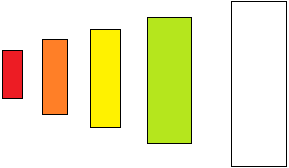
\includegraphics[scale=0.35]{images/4.png}}
\end{figure}

\par\medskip

\textbf{Contents}\par
The score of this section is given simply by the score evaluated by the \textit{Information Overload} heuristic which is \textbf{4.5}. \par
So basing only this heuristic, content of the website is almost fully satisfied. Improvements could be done, but fixes will be minimal.

\begin{figure}[H]
  \centering
  \makebox[\linewidth]{
    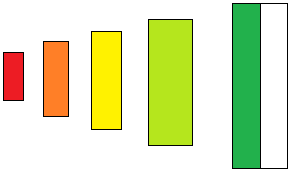
\includegraphics[scale=0.35]{images/4.5.png}}
\end{figure}


\par\medskip
\pagebreak
\textbf{Layout}\par
The layout score is given by the mean of 5 aspects analyzed in the section \ref{Layout}. \par
The final result is: 
(4 + 4 + 4 + 4 + 3)/5 = 3.8 \\
\textit{which can be approximated to} \textbf{4}\par
Basing on the result, layout of the website it's pretty well designed, but with some critical issues that should be fixed in order to have the best experience.

\begin{figure}[H]
  \centering
  \makebox[\linewidth]{
    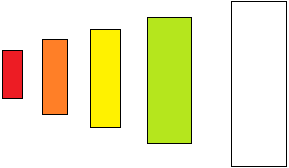
\includegraphics[scale=0.35]{images/4.png}}
\end{figure}


\subsection{Nielsen}
Instead, the evaluation with this set of heuristics is made by making the average of all the six heuristcs analyzed:
(2 + 4 + 3.5 + 4 + 5 + 4.5)/6 = 3.8 \\
\textit{which can be approximated to} \textbf{4}.\par

\begin{figure}[H]
  \centering
  \makebox[\linewidth]{
    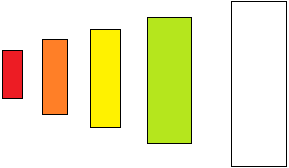
\includegraphics[scale=0.35]{images/4.png}}
\end{figure}

\section{Comments}
As evidenced by the results obtained from the analysis carried out by our team, the site has high standards obtained on the various fields evaluated and, although there are criticalities widely described in the appropriate sections, as a whole it is functional, well done and adequate for its purpose of use; our work concerning the Inspection of the web site therefore ends with an overall satisfactory score.





\end{document}